\subsection{Die Wertschöpfungskette}\label{wsk}
Damit der Weg von Entwicklung, über Bereitstellung und letztendlichen Kauf einer Software nachvollzogen werden kann, werden einige im Business Model identifizierten Schlüsselpartner in Abbildung \hyperref[img:supplychain]{7} im Kontext einer Supply Chain dargestellt. Der Prozess startet bei Software Providern, welche eine Idee für eine Software haben und diese umsetzen. Hierzu ist möglicherweise die Zusammenarbeit mit Service Providern notwendig. Die entwickelte Software wird an den Software Shop weitergeleitet und dieser stellt sie entweder im Shop bereit oder nicht. Abschließend können Fahrzeughalter Software über eine kabellose Schnittstelle wie das Internet herunterladen, wobei Mobilfunkbetreiber der Mittelsmann für Mobilfunknetze darstellen. Die Wertschöpfungskette ist als detailliertere Sicht des "\textit{Software Shops}" (Abbildung \hyperref[img:supplychain]{7}) zu sehen. Sie stellt die Entscheidungen und Schritte dar, die eine Software von der Lieferung des Software Providers \textbf{(IN)} bis zum Download im Shop \textbf{OUT} durchlaufen und bestehen muss.
\begin{figure}[!h]
	\centering
	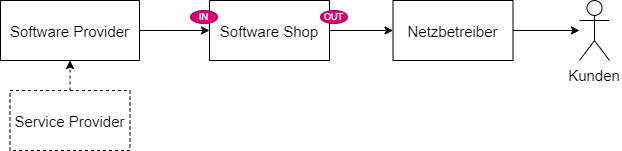
\includegraphics[width=0.9\columnwidth]{pictures/konzept-supplychain.png}
	\label{img:supplychain}
	\caption{Supply Chain von Software}
\end{figure}\\
Nach Porter ist die Wertschöpfungskette in primäre und unterstützende Aktivitäten aufzuteilen.\cite{wsk}Primäre Aktivitäten "liefern [dabei] einen direkten wertschöpfenden Beitrag zur Erstellung eines Produktes"\cite[]{wsk} und Unterstützende Aktivitäten sind als "notwendige Voraussetzung zu Erstellung der Produkte"\cite[]{wsk}zu sehen. Sie sind im Rahmen aller Primäraktivitäten aktiv und beeinflussen die Qualität des Produktes \cite[Vgl.]{wsk2}. Abbildung \hyperref[img:wsk]{8} ordnet die in Kapitel \ref{key_activities} identifizierten Bausteine den Aktivitäten einer Wertschöpfungskette zu - die dort festgelegte Gruppierung der Schlüsselaktivitäten wird beibehalten.

\subsubsection{Primäre Aktivitäten}
Es gibt fünf primäre Aktivitäten. Die erste Aktivität ist die Beschaffung und Lagerung von Materialien, in diesem Fall von Softwares, welche als \textbf{Eingangslogistik} bezeichnet wird \textit{(Links unten im Bild)}. Im Kontext dieser sind zwei wichtige Bausteine zu erwähnen:
\begin{itemize}
	\item[] \hspace{-0.6cm}\textbf{Verifikation der Software-Sicherheit}\\ \label{security}
	Sämtliche Softwares die dem Shop hinzugefügt werden sollen, müssen zunächst diverse Sicherheitschecks bestehen. Zum einen sollten Softwares hinsichtlich aufgenommener und gespeicherter Daten überprüft werden. Je nach Land gelten unterschiedliche Datenschutzrichtlinien, welche zu beachten sind um die Privatsphäre von Fahrzeughaltern zu schützen. Weiterhin muss festgestellt werden, dass durch die neue Software keine Sicherheitslücken bei der Fahraufgabe entstehen. Dies kann durch Simulationen getan werden, wie in Kapitel \ref{technische_konzepte} gezeigt wird.\\
	Es ist sinnvoll, ein Sicherheitskonzept zu entwickeln in welchem die zum einen die aufgezählten als auch weitere mögliche Sicherheitslücken von Softwares geprüft werden. Das Ziel der Sicherheitsverifikation ist letzten Endes, dass durch neues Softwares keine Gefahren für die Fahrzeuginsassen entstehen. 
	
	\item[] \hspace{-0.6cm} \textbf{Klassifizierung von Software}\\
	Erfüllt eine Software die Sicherheitsrichtlinen, wird sie anschließend Klassifiziert. Die Klassifizierung von Software soll die Suche und Darstellung dieser im Shop unterstützen, in dem einer Software diverse Meta-Daten hinzugefügt werden. Diese können im Shop einerseits als Such-Filter verwendet werden, einzelne können auc angeben wie gut/schlecht eine Software ist. Ein beispielhaftes Konzept  wird in Kapitel \ref{sw_klassifizierung} erarbeitet.
\end{itemize}
\begin{figure}[!h]
	\hspace{-1.5cm}
	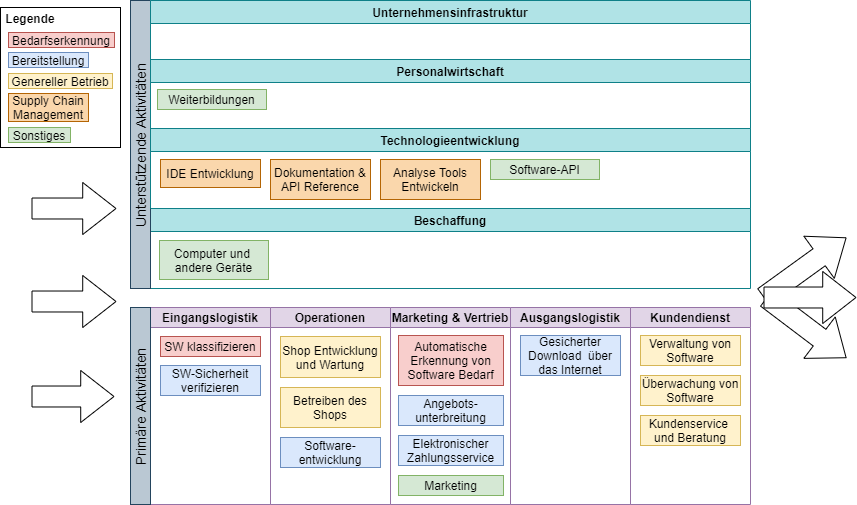
\includegraphics[width=1.2\columnwidth]{pictures/konzept-wsk.png}
	\label{img:wsk}
	\caption{Die wichtigsten Bausteine einzelner Aktivitäten der Wertschöpfungskette}
\end{figure}
Nach erfolgreichen Durchlaufen der Eingangslogistik folgen die Aktivitäten der \textbf{Operation}. Im Rahmen dieser werden die verifizierten und klassifizierten Softwares dem Shop hinzugefügt und verwaltet. Die Operationen sind die Aufgaben des Unternehmens, in welchen der eigentliche Mehrwert für die Kunden geschaffen wird. 
\begin{itemize}
	\item[] \hspace{-0.6cm} \textbf{Shop (Weiter-)Entwicklung und Wartung}\\
	Der Software Shop ist das Herz des Unternehmens, ohne welchen dessen Existenz nicht möglich ist. Die (Weiter-)Entwicklung und Wartung des Shops ist daher eine der Kernaufgaben des Unternehmens. Änderungen und neue Funktionen betreffen entweder das Front-End oder das Back-End des Shop. Das Front-End ist die grafische Oberfläche \textit{(Mensch Maschine Schnittstelle)}, die letzten Endes von den Fahrzeughaltern bedient wird. Bei der Front-End-Entwicklung kann die Verwendung des User-Centered-Designs zu einer Verbesserung von UI und UX \textit{(User-Experience)} führen. Das Back-End ist für den Fahrzeughalter nicht sichtbar - es \textbf{verarbeitet Kauf- und Suchanfragen für Softwares} und muss dementsprechend schnell und effizient sein, um eine große Menge derartiger Anfragen zu bewältigen. Da der Shop viel Software umfasst, die von Software Providern entwickelt wurde, sollte bei der (Weiter-)Entwicklung des Shops auf Kritik, Verbesserungsvorschläge und Wünsche dieser eingegangen werden. Auch die übrige \textit{Community} (OEMs, Fahrzeughalter, Flottenbetreiber) sollte hier einbezogen werden.\\
	Neben der (Weiter-)Entwicklung des Shops, muss auch die bereits existierende Plattform zusätzlich gewartet werden. Dies umfasst den Austausch von unzuverlässiger Hardware, aber auch das schnelle beheben von Bugs, die im Shop aufgetreten sind sowie die kontinuierliche Überwachung der Datenbanken, Server etc.

	\item[] \hspace{-0.6cm}\textbf{Betreiben des Shops}\\	
	Damit der Shop betrieben werden kann, müssen durch die Eingangslogistik klassifizierte und verifizierte Softwares dem Shop hinzugefügt oder aus diesem entfernt und eingehende Download-Anfragen verarbeitet werden. Außerdem müssen Softwares die vermehrt von Fahrzeughaltern gemeldet wurden, müssen überprüft und gegebenenfalls aus dem Shop entfernt werden. Damit im Shop keine Inhalte \textit{(Softwares, Bewertungen von Softwares)} vorkommen, die diskriminierend, rassistische oder auf eine andere Art \& Weise Menschenrechts-verletzend sind, sollten diese sofort aus dem Shop entfernt werden\\.
	Softwares die im Laufe der Zeit als \glqq besonders gut\grqq aufgefallen sind, können ein Siegel \glqq Empfehlung der Redaktion\grqq erhalten. Dieses soll die Qualität einer Software hervorheben und Fahrzeughalter bei der Kaufentscheidung unterstützen. 
			
	\item[] \hspace{-0.6cm} \textbf{Eigene Softwareentwicklung}\\
	Neben der Bereitstellung von Software anderer Software Provider ist auch die eigene Entwicklung und Bereitstellung von Software im Shop möglich. Einerseits stellt der Verkauf eigener Software weitere Einnahmequelle für das Unternehmen, andererseits lässt sich durch den Verkauf einer guten, günstigen Software das Image des Shops steigern. 
\end{itemize}
Die vorgestellten Aufgaben stellen Voraussetzungen dar, welche für den Verkauf von Software notwendig sind. Da der Shop bereits auf Fahrzeugen installiert ist \textit{(siehe Abschnitt \ref{key_partners})}, müssen Fahrzeughalter anschließend zum Kauf bewegt werden. Dies passiert durch den dritten Aufgabenbereich der Wertschöpfungskette, dem \textbf{Marketing und Vertrieb} von Software.
\begin{itemize}
	\item[] \hspace{-0.6cm} \textbf{Automatische Erkennung von Softwarebedarf}\\
	Um Fahrzeughalter beim Kauf von Software zu unterstützen soll sichergestellt werden, dass gekaufte Softwares auch tatsächlich benötigt werden. Hierzu soll der Softwarebedarf eines Fahrzeug automatisch anhand von Fahrt- und Fahrzeugdaten identifiziert und dem Fahrzeughalter vorgeschlagen werden. Es gibt diverse Möglichkeiten den Softwarebedarf eines Fahrzeugs automatisch zu bestimmen:\\	
	\subitem \textbf{Suche anhand einer einzelnen Situation} \\
		Diese Suche wird in Kapitel \ref{2.3} beschrieben. Das Ergebnis der Suche enthält entweder \textbf{keine} oder genau \textbf{eine} Software, welche eine zuvor identifizierte Lücke der autonomen Fahrfunktionen abdeckt. Die Suche soll automatisch erfolgen und die Vorschläge werden im Shop angezeigt.
		
	\subitem \textbf{Routen-Basierte Suche nach Software}\\
		Ebenfalls in Kapitel \ref{2.3} beschrieben, erfolgt diese Suche vor Fahrtantritt und durchgeführt wenn das Fahrzeug bzw. der Fahrzeughalter kurz davor ist eine nicht häufig zurückgelegte Strecke zu Fahren. Die Ergebnisse der Suche werden in die Routenplanung integriert und dem Fahrzeughalter wie in Kapitel \ref{2.3} beschrieben vor Fahrtantritt vorgeschlagen.
		
	\subitem \textbf{Shop-Basierte Suche \textit{(Shop-Auswahl)}}\\
		Wird eine Software im Shop ausgewählt die dem Fahrzeughalter noch nicht vorgeschlagen wurde, kann dieser bestimmen lassen ob und wenn ja zu welchem Umfang die jeweilige Software das Fahrspektrum des Fahrzeugs erweitert. Das Ergebnis der Anfrage stellt eine gute Entscheidungsgrundlage für den Kauf der Software dar, da dem Fahrzeughalter so der tatsächliche \textit{persönliche} Nutzen einer Software präsentiert wird.
		
	\subitem \textbf{Umgebungsbedingte Softwaresuche}\\
		Die Umgebungssuche ist eine Weiterentwicklung der in Kapitel \ref{2.3} dargestellten \textit{Suche aus Basis der Fahrtenhistorie.} Die Idee dieser ist es, dass dem Fahrzeughalter Softwares vorgeschlagen werden die andere Fahrzeughalter in der Region vermehrt installiert haben. Die Umgebungs-Suche wird in Kapitel \ref{umgebungssuche} im Detail erläutert.
	
	Abhängig davon, ob passende Softwares gefunden wurden oder nicht, werden sie dem Fahrzeughalter vorgeschlagen. Durch den Prozess wird die Kundenzufriedenheit gesteigert, als auch mehrere Nutzenversprechen gefördert \textit{(NV-2, NV-3, NV-4, NV-5)}. Neben Suchalgorithmen die dem Fahrzeughalter Softwarevorschläge unterbreiten, können auch Service Provider einem Fahrzeug eine Software vorschlagen. Dies ist notwendig, wenn der Fahrzeughalter einen Service nutzen will für welchen eine bestimmte Software auf dem Fahrzeug installiert sein muss.

	\item[] \hspace{-0.6cm} \textbf{Angebotsunterbreitung}\\
	Wird anhand einer der zuvor aufgelisteten Suchen festgestellt, dass eine bestimmte Software die Fahrfunktionen eines Fahrzeugs sinnvoll erweitern kann, sollte diese dem Fahrzeughalter vorgeschlagen werden. Im Kontext der Angebotsunterbreitung ist der Zeitpunkt wichtig, zu welchem die Software dem Fahrer vorgeschlagen wird. Ein Konzept für die Bestimmung eines geeigneten Zeitpunkts zum Vorschlagen eines Software wurde in Kapitel \ref{3.3} erläutert.
	
	\item[] \hspace{-0.6cm} \textbf{Bereitstellung elektronischer Zahlungsschnittstellen}\\
	Um den Kauf einer Software abschließen zu können, müssen Fahrzeughalter den Kaufpreis über eine elektronische Zahlungsschnittstelle bezahlen können. Hierzu sollten bestenfalls mehrere gängige Zahlungsschnittstellen \textit{(MasterCard, PayPal, EC-Cash o.A.)} mit dem Shop verknüpft werden, um so mehr Fahrzeughaltern den Kauf zu ermöglichen. Um weitere eigene Umsätze zu generieren, kann hier auch eine eigene Zahlungsschnittstelle eingebaut werden. Fahrzeughalter können zur Verwendung dieser gebracht werden, indem der Kauf mittels dieser Schnittstelle beispielsweise günstiger oder schneller ist.\\
	
	\item[] \hspace{-0.6cm} \textbf{Marketing}\\
	Wie im Business Model beschrieben, ist der Umfang des Marketings maßgebend für den Erfolg des Shops. Die Kampagnen sollten auf möglichst vielen Kanälen zu sehen sein und dabei möglichst viele Alters- und Kundengruppen ansprechen. Vor allem die Vermarktung über Social Media Kanäle ist ratsam. Es kann Sinnvoll sein "Markenbotschafter" zu finden, die Content für Social Media Plattformen entwerfen. Coca Cola hat dies beispielsweise erfolgreich mit Coke TV\footnote{\url{https://www.youtube.com/channel/UCTfwo-EWSD-8hZ7F8HG_qJg}, Aufgerufen am 14. Juni 2020} getan.
\end{itemize}
Damit die von Fahrzeughaltern gekauften Softwares letztendlich auch an Fahrzeuge verteilt werden können, muss die \textbf{Ausgangslogistik} strukturiert werden welche festlegt, über welche Distributionskanäle Software verteilt wird.
\begin{itemize}
	\item[] \hspace{-0.6cm} \textbf{Gesicherter Download über das Internet}\\
	Die Bereitstellung bezahlter Softwares wird mit dem Download abgeschlossen. Dieser Download soll orts- und zeitunabhängig sein und muss über eine sichere Schnittstelle erfolgen. Um dies zu gewährleisten, sollte der Ausbau von Kommunikationsnetzwerken \textit{(bspw. 5G)} gefördert werden und eine sichere Architektur für den Server entworfen werden \textit{(Uptane, Kapitel \ref{uptane})}. Da durch den Download von Software über das Internet hohe Kosten für Fahrzeughalter entstehen können, sollten Kooperationen mit Mobilfunkanbietern abgeschlossen werden, durch welche die Kosten skalierbar gehalten und die Kundenzufriedenheit gesichert werden kann.
\end{itemize}
Um die Kundenzufriedenheit weiter zu stärken, müssen auch nach dem Kauf für den Kunden wertschöpfende Aktivitäten durchgeführt werden. Diese werden dem letzten Schritt der Wertschöpfungskette, dem \textbf{Kundendienst}, zugeordnet.	
\begin{itemize}
	\item[] \hspace{-0.6cm} \textbf{Verwaltung von gekaufter Software}\\
	Damit Fahrzeughalter wissen, welche Softwares sie gekauft, geliehen oder gemietet haben soll für sie die eigenständige Verwaltung von Software im Shop möglich sein. Fahrzeughalter behalten hierdurch den Überblick über ihr Fahrzeug und können Softwares entfernen oder hinzufügen.
	
	\item[] \hspace{-0.6cm} \textbf{Überwachung installierter Software}\\
	Um Fahrzeughaltern vor Augen zu führen, welche Softwares tatsächlich vom Fahrzeug genutzt werden und welche nicht, sollten diese Einblick in eine Art Überwachung der Software haben. Hier können grundlegende Statistiken geführt werden wie
	\begin{itemize}
		\item die durchschnittliche Nutzungsdauer einer Software je Woche
		\item das Datum, an welchem die Software das letzte mal genutzt wurde
		\item oder eine Liste, in welcher zu sehen ist welche Softwares an welchem Tag der Woche vermehrt genutzt werden.
	\end{itemize}
	Aufgrund der steigenden Bedeutung des Datenschutzes könnte auch eine Ansicht erstellt werden, welche zeigt welche Daten von Softwares erhoben werden. Hierdurch könnte das Vertrauen von Kunden gestärkt werden \textit{(Oder auch nicht, je nach dem welche und wie viele Daten erhoben und gespeichert werden)}.
	
	\item[] \hspace{-0.6cm} \textbf{Kundenservice und Beratung}\\
	Um vor allem die Bindung zu älteren Kunden zu stärken, kann das einrichten einer Telefonischen Beratung sinnvoll sein. Vor allem bei der Ersteinrichtung eines Fahrzeugs kann die telefonische Unterstützung von Fahrzeughaltern positive Auswirkungen auf die Kundenzufriedenheit haben. Auch alternative, vorwiegend digitale Varianten Fahrzeughalter bezüglich Sofwtares zu beraten kann einen Mehrwert für diese bieten. Durch das entwickeln von Nutzerforen oder der Möglichkeit, Softwares im Shop zu bewerten \textit{(1-5 Sterne + Kommentar)} können Fahrzeughalter sich gegenseitig beraten.
\end{itemize}
\textbf{Überblick}\\
Die fünf Aktivitäten der Wertschöpfungskette schaffen Mehrwerte für Fahrzeughalter. Wird eine Software von einem Software Providern beim Softwareshop \glqq eingereicht\grqq, wird sie für den Verkauf an Fahrzeughalter vorbereitet. Jeder einzelne Schritt der Wertschöpfungskette trägt dazu bei, das Fahrzeughalter letztendlich selbstständig Softwares kaufen können, die sie tatsächlich benötigen. Während all diese Schritte durchlaufen werden, fügen die \textit{unterstützenden Aktivitäten} stetig Mehrwerte zur Wertschöpfung hinzu und sind daher\textit{indirekt am Erfolg beteiligt}. Im folgenden werden diese vorgestellt und ihre Rolle im Ablauf der Wertschöpfungskette verdeutlicht.

\subsubsection{Unterstützende Aktivitäten}\label{unterstd_activities}
Es gibt vier Unterstützende Aktivitäten. Angefangen bei der Schaffung einer gut aufgebauten \textbf{Unternehmensinfrastruktur}, welche alltägliche Problematiken beheben und Zeit sparen kann. Zu dieser gehört ein gute Anbindung zur Außenwelt, schnelles Internet und weiteres.\footnote{quelle} Neben der Schaffung einer guten Unternehmensinfrastruktur hat auch die \textbf{Personalwirtschaft} \textit{(Human-Resource-Management)} einen starken Einfluss auf den Erfolg des Unternehmens. Sie beschreibt wichtige, die Mitarbeiter unterstützende Strukturen und Regelungen des Unternehmens, wie zum Beispiel Weiterbildungen und Workshops.
\begin{itemize}
	\item[] \hspace{-0.6cm} \textbf{Weiterbildungen}\\
	Die kontinuierliche Weiterbildung der Mitarbeiter ist für den Erfolg des Shops überaus wichtig. Weiterbildungen müssen nicht Zwangsweise in dem jeweiligen Fachbereich des Mitarbeiters liegen, sondern können auch neue Aspekte beleuchten. So können Entwickler einerseits gemeinsamen neue Programmiersprachen \& -frameworks lernen, anderseits können auch andere \glqq Skills\grqq beigebracht oder Aktivitäten \textit{(bspw. Sport)} miteinander durchgeführt werden, welche die Team-Chemie steigern. Die Schaffung einer guten Work-Life-Balance kann die Produktivität der Mitarbeiter erhöhen\cite[Vgl. S.4]{wlb} und somit den Erfolg des Shops nachhaltig unterstützen.
	
\end{itemize}
Für ein (digitales) Unternehmen ist die stetige \textbf{Technologieentwicklung} wichtig und kann wegweisend für den Erfolg des Unternehmens sein.\ref{quelle} Zu dieser gehört nicht nur die Schaffung von Werten für die innerbetriebliche Wertschöpfungskette, sondern auch die Supply Chain übergreifend Unterstützung der Partner und Kunden.

\begin{itemize}
	\item[] \hspace{-0.6cm} \textbf{IDE Entwicklung}\\
	Damit Software Provider bei der Entwicklung von Softwares unterstützt werden, ist die Bereitstellung einer eigens entwickelten Entwicklungsumgebung\textit{(IDE)} sinnvoll. 
	Diese IDE kann Features und Tools umfassen, welche explizit für die Entwicklung von (Fahrzeug-) Softwares entwickelt wurden. Durch integrierte Simulatoren, Sicherheitschecks und andere Tools könnte der Weg von Idee über Entwicklung hinzu Bereitstellung im Shop verkürzt und vereinfacht werden. Ein Vergleich aus der Realität ist Android Studio\footnote{https://developer.android.com/studio} aber auch die Eclipse IDE, welche in Zusammenarbeit mit Unternehmen aus der ganzen Welt entwickelt wird\footnote{\url{https://www.eclipse.org/org/}, Aufgerufen am \today} und die Einbindung von Plugins einfach gestaltet.
	
	\item[] \hspace{-0.6cm} \textbf{Dokumentation und API-Reference}\\
	Die Entwicklung von Software wird zusätzlich durch die Bereitstellung einer ausführlichen API-Reference sowie technischen Dokumentation (mit Beispielen) positiv unterstützt. Eine API-Reference sollte alle Funktionenen des Frameworks ausführlich beschreiben und im Nutzungskontext vorstellen. Diagramme unterstützen zusätzlich das Verständnis der API. Um die Entwicklung neuer Softwares voranzutreiben und zu vereinfachen ist es sinnvoll eine Einführung \textit{('Getting Started Guide')} für diese bereitzustellen. Google stellt in diesem Kontext das \textit{Android Jetpack}\footnote{\url{https://developer.android.com/jetpack}, Aufgerufen am \today} sowie weitere Dokumentationen mit Anleitungen und Videos zur Verfügung.\footnote{\url{https://developer.android.com/guide}, Aufgerufen am \today}. Auch und vor allem sollten hier die Sicherheitskriterien, welche im Kontext der Wertschöpfungskette in Abschnitt \textbf{Eingangslogistik} erwähnt wurden, vorgestellt werden. 
	
	\item[] \hspace{-0.6cm} \textbf{Entwicklung von Analyse-Tools}\\
	Um Software Provider zusätzlich bei der (Weiter-)Entwicklung zu unterstützen, können Analyse-Tools entwickelt werden, welche die Entwickler Entwicklung unterstützen. Analysierte Statistiken können generelle Kennzahlen\textit{(Nutzung in H je Tag)} aber auch spezifischere Werte \textit{(Button-Clicks)} sein, durch welche Entwickler dazu in der Lage sind, ihre Software zu verbessern.
	
	\item[] \hspace{-0.6cm} \textbf{API-Entwicklung}\\
	Damit Software Provider bestimmte Systeme von Fahrzeugen ansteuern können, müssen APIs für die jeweiligen Systeme eines Fahrzeugs entwickelt werden. Über diese können Daten der Systeme ausgelesen oder eingefügt werden. Da künftig hergestellte Fahrzeuge sehr wahrscheinlich neuartige Technologien und Feature enthalten die heutzutage noch nicht existieren, müssen die APIs im Laufe der Zeit immer weiter angepasst bzw. erweitert werden.\\\\
	\textbf{ANPASSEN und API-KONZEPT EINBAUEN!}\\
	Damit \glqq alte\grqq Fahrzeuge weiterhin von einer Software gesteuert werden können, müssen die alten APIs aber bestehen bleiben. In Android wird diese Problematik sinnvoll durch das \textit{"API-Level"} gelöst: Jede Android Version hat ein eigenes \textit{API-Level}. Je höher das Level, desto höher auch die Android Version. Ein Smartphone mit API-Level 23 \textit{(Android 6.0)} kann alle Funktionen und Methoden \textit{"tieferer"} APIs nutzen, nicht aber die \textit{"höherer"} APIs \textit{(>23)}. Jede App hat eine \textit{minimale API-Version} welche festlegt, welches API-Level das Endgerät mindestens haben muss. Im Kontext von Fahrzeugen ist es vorstellbar, dass jedes Teilsystem eines Fahrzeugs ein eigenes mininmales API-Level hat. Softwares dadurch nur auf Fahrzeugen installiert werden, welche den Anforderungen der Software entsprechen. 
\end{itemize}

Die letzte unterstützende Aktivität ist die \textbf{Beschaffung}. Ihre Aufgabe ist, dass alle Mitarbeiter mit den nötigen Materialien wie Computern, Tastaturen, Stiften oder anderem versorgt werden.\\\\